%% 
%% Copyright 2007, 2008, 2009 Elsevier Ltd
%% 
%% This file is part of the 'Elsarticle Bundle'.
%% ---------------------------------------------
%% 
%% It may be distributed under the conditions of the LaTeX Project Public
%% License, either version 1.2 of this license or (at your option) any
%% later version.  The latest version of this license is in
%%    http://www.latex-project.org/lppl.txt
%% and version 1.2 or later is part of all distributions of LaTeX
%% version 1999/12/01 or later.
%% 
%% The list of all files belonging to the 'Elsarticle Bundle' is
%% given in the file `manifest.txt'.
%% 
%% Template article for Elsevier's document class `elsarticle'
%% with harvard style bibliographic references
%% SP 2008/03/01

%\documentclass[preprint,12pt,authoryear]{elsarticle}
\documentclass[preprint,12pt]{elsarticle}
%% Use the option review to obtain double line spacing
%% \documentclass[authoryear,preprint,review,12pt]{elsarticle}

%% Use the options 1p,twocolumn; 3p; 3p,twocolumn; 5p; or 5p,twocolumn
%% for a journal layout:
%% \documentclass[final,1p,times,authoryear]{elsarticle}
%% \documentclass[final,1p,times,twocolumn,authoryear]{elsarticle}
%% \documentclass[final,3p,times,authoryear]{elsarticle}
%% \documentclass[final,3p,times,twocolumn,authoryear]{elsarticle}
%% \documentclass[final,5p,times,authoryear]{elsarticle}
%% \documentclass[final,5p,times,twocolumn,authoryear]{elsarticle}

%% For including figures, graphicx.sty has been loaded in
%% elsarticle.cls. If you prefer to use the old commands
%% please give \usepackage{epsfig}

\input symbols

%% The amssymb package provides various useful mathematical symbols
\usepackage{amssymb}
%% The amsthm package provides extended theorem environments
%% \usepackage{amsthm}

%% The lineno packages adds line numbers. Start line numbering with
%% \begin{linenumbers}, end it with \end{linenumbers}. Or switch it on
%% for the whole article with \linenumbers.
%% \usepackage{lineno}

\journal{Nuclear Physics B}

\begin{document}

\begin{frontmatter}

%% Title, authors and addresses

%% use the tnoteref command within \title for footnotes;
%% use the tnotetext command for theassociated footnote;
%% use the fnref command within \author or \address for footnotes;
%% use the fntext command for theassociated footnote;
%% use the corref command within \author for corresponding author footnotes;
%% use the cortext command for theassociated footnote;
%% use the ead command for the email address,
%% and the form \ead[url] for the home page:
%% \title{Title\tnoteref{label1}}
%% \tnotetext[label1]{}
%% \author{Name\corref{cor1}\fnref{label2}}
%% \ead{email address}
%% \ead[url]{home page}
%% \fntext[label2]{}
%% \cortext[cor1]{}
%% \address{Address\fnref{label3}}
%% \fntext[label3]{}

\title{Neutrino oscillations: the rise of the PMNS paradigm}

%% use optional labels to link authors explicitly to addresses:
%% \author[label1,label2]{}
%% \address[label1]{}
%% \address[label2]{}

\author{St\'ephane Lavignac}

\address{IPhT, CEA Saclay, 91191 Gif-sur-Yvette CEDEX, France}

\author{Marco Zito}

\address{IRFU/SPP, CEA Saclay, 91191 Gif-sur-Yvette CEDEX, France}

\begin{abstract}
%% Text of abstract
This is the abstract
\end{abstract}

\begin{keyword}
%% keywords here, in the form: keyword \sep keyword

%% PACS codes here, in the form: \PACS code \sep code

%% MSC codes here, in the form: \MSC code \sep code
%% or \MSC[2008] code \sep code (2000 is the default)

\end{keyword}

\end{frontmatter}

%% \linenumbers

%% main text
\section{Introduction}
\label{sec:intro}


\section{Theory and phenomenology of oscillations 15 pg SL}
\label{sec:th}

\subsection{Preliminary}

Lagrangian NC and CC, nu in SM, m ?

\subsection{Basis}

U PMNS : D vs M, oscillation independent of D/M
vacuum N=2 N=3

\subsection{matter}
n=const  $\rightarrow$ MH determination 

\subsection{MSW}
adiabatic regime


\subsection{CP violation}

CP violation vacuum (+ CP with matter ?)


\section{Oscillation parameters: current status 30pg}
\label{sec:status}

\subsection{The solar sector: SK, SNO, KamLAND  (SL)}

reactions + spectrum nu solar (plot)

Davis first indication deficit Ga/Sage confirmation, E dependance

SK mesure spectrum vs E plot

SNO mesure NC/CC  $\rightarrow$ Phi (nu other)/Phi(nue) plot

Kamland confirmation artificial beam (vacuum) E/L oscillation plot precision meas. Dm**2 $\rightarrow$ excludes LOW  $\rightarrow$ LMA 

(MSW interpretation) Borexino  mesure various components of the spectrum (Be, CNO) $\rightarrow$ confirmation MSW (upturn) day night effect


\subsection{The atmospheric sector: SK, K2K, Minos, T2K  (MZ)}

In this subsection we will describe the status of the so called atmospheric neutrino oscillations, i.e. the 3-2 oscillations that were first discovered in the study of atmospheric neutrinos and later were precisely measured with the use of long baseline neutrino beams.   


\subsubsection{The atmospheric neutrino flux}

The atmosphere is constantly bombarded by primary cosmic rays, composed mainly of protons, with a smaller component of $\alpha$ particles and heavier nuclei. The interaction of these particles with atomic nuclei in the atmosphere produces hadronic showers composed mainly of pions and kaons. The decay of these mesons according to 
$\pi^+ \rightarrow \mu^+ \nu_\mu$ followed by 
$\mu^+ \rightarrow e^+ \nu_e \bar{\nu}_\mu $,
$K^+ \rightarrow \pi^+ \nu_\mu$ and $K_L \rightarrow \pi^+ e^- \nu_e$
together with their charge conjugated processes, produces a flux of $\nu_\mu$ and $\nu_e$ with a steeply falling power-law spectrum (Fig. \ref{fig:nuatmflux}). 


\begin{figure}[htbp]
\begin{minipage}[c]{.46\linewidth}
%\begin{minipage}[c]
   	      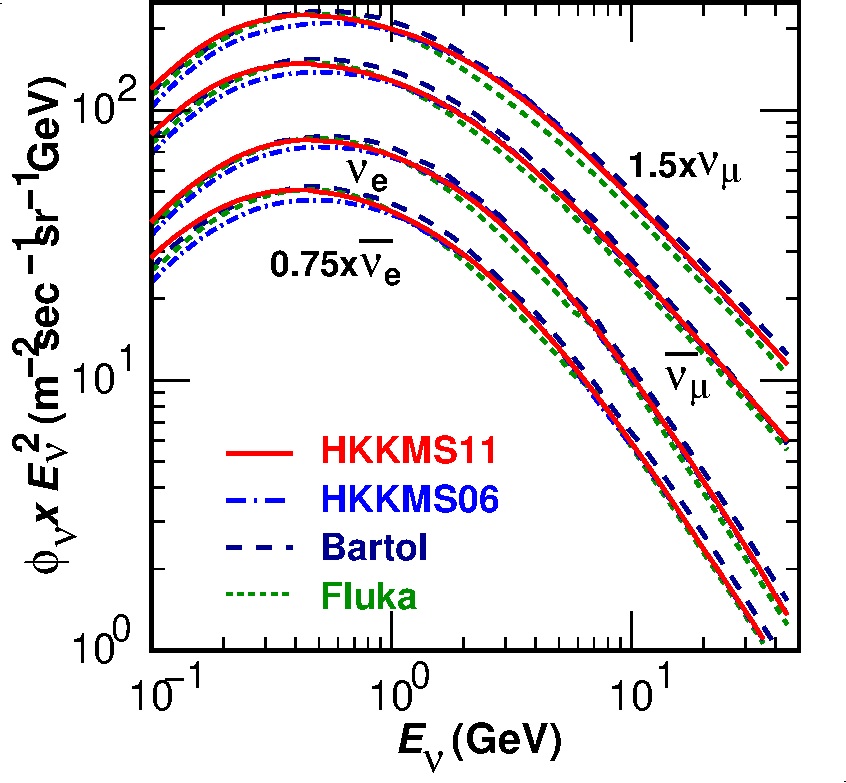
\includegraphics[width=0.9\linewidth]{figures/fig7a-c.pdf}
   \end{minipage} \hfill
   \begin{minipage}{.46\linewidth}
      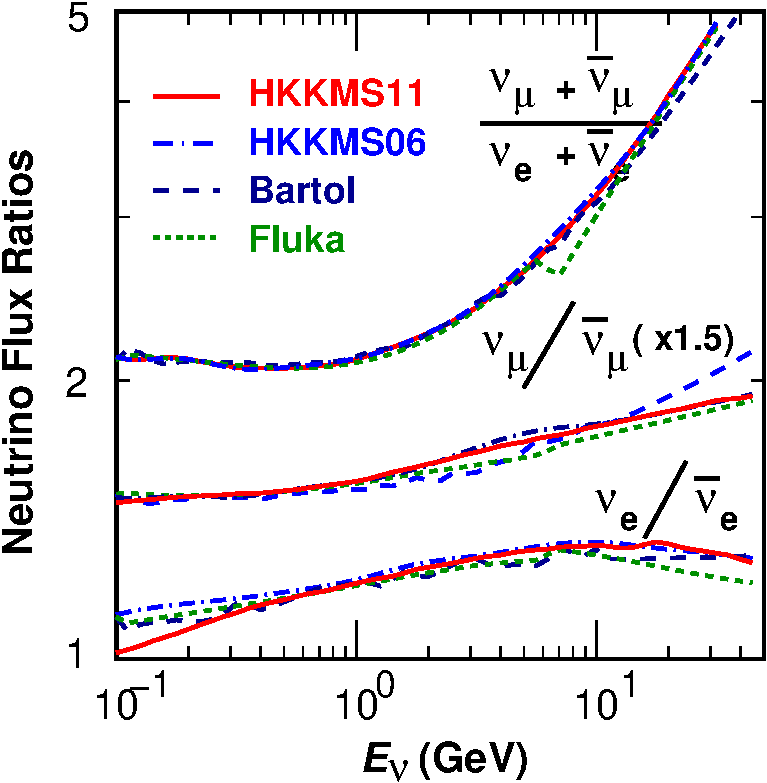
\includegraphics[width=0.9\linewidth]{figures/fig7b-c.pdf}
   \end{minipage}
    \caption{The flux of atmospheric neutrinos (left) and several flux ratios (right) \cite{ref:midori}. }
 \label{fig:nuatmflux}
\end{figure}


The calculation of this neutrino flux \cite{ref:Ga2002} relies on the knowledge of the primary flux and composition, of the Earth magnetic field, and of the hadro-production cross-section. Recent studies \cite{ref:midori,ref:barr,ref:fluka} taking into account 3D effects and recent measurements of the hadro-production cross-sections largely improve on previous efforts and reach precisions of 7-8 \% for the flux in the 1-10 GeV range. It should be noticed that the ratio $N(\nu_\mu + \bar{\nu}_\mu)/N(\nu_e + \bar{\nu}_e)$ is predicted with a much better precision of a few \% as several systematic uncertainties cancel in this ratio. In the limiting case where all the muons from pion decays decay themselves in flight, this ratio is close to 2, as can be easily deduced from the decay processes mentioned above.

\subsubsection{The early days, the up-down asymmetry and controversy}

The study of atmospheric neutrinos started in the 1960: two experiments in very deep mines, in South Africa \cite{ref:reinesAtm} and in India \cite{ref:achar}, observed muons produced by their interactions. 
In the 1980, several massive underground experiments, mainly motivated by the search for the proton decay predicted by Grand Unification theories, started collecting data. These experiments needed to study in detail atmospheric neutrino interactions as they constitute a background for proton decay searches.

In 1988, Kamiokande reported a deficit in the number of $\nu_\mu$ of events, while the number of $\nu_e$ events agreed with the prediction. This started the so-called atmospheric neutrino anomaly. This deficit was also observed by the IMB experiment and later by MACRO and SOUDAN-2, while Fr\'ejus and NUSEX observed no deficit. 


\subsubsection{The evidence for atmospheric neutrino disappearance}
%from Super-Kamiokande}


The situation evolved rapidly with the advent of Super-Kamiokande, that started data-taking in 1996. Super-Kamiokande is very large water Cherenkov detector located in the Mozumi mine (Gifu prefecture, Japan), under a 1000 m rock overburden, equivalent to 2700 m of water. It is a stainless steel tank (41.4 m high, 39.3 m diameter) containing 50 kt of ultra-pure water. The detection volume is partitioned in an outer detector, composed of 1885 8 inch PMTs, and an inner detector with 11146 20 inch PMTs. The fiducial volume is 22.5 kt. Super-Kamiokande could rapidly accumulate a rather large data set of atmospheric neutrinos, measuring the direction of the produced lepton, its energy for fully contained events and their nature. Above a few hundred MeV/c, the direction of the produced lepton is strongly correlated to the direction of the incoming neutrino.  

In 1998, the Super-Kamiokande collaboration presented their first analysis of atmospheric neutrinos~\cite{ref:skatm98}, in particular the distributions of zenith angle for $ \nu_\mu$ and $\nu_e$ event selections (see Fig.~\ref{fig:sk-atm} for an updated distribution) based on 33 kton year. This was the first compelling evidence for neutrino oscillations as the explanation of the previously mentioned anomaly.  

Indeed the neutrino path from the production to the detection varies from 15 km for down-going neutrinos (cosine of the zenith angle equal to 1) to more than 12000 km for up-going neutrinos having traversed the whole Earth (cosine of the zenith angle equal to -1), thereby probing a large span of possible oscillation lengths. 

In a two neutrino scenario, the $\nu_\mu$ disappearance is governed by $\sin^2 (2 \theta) \sin^2 (4 \Delta m^2 L /E)$, where $\theta$ is the relevant mixing angle and $\Delta m^2$ the squared-mass difference of the mass eigenstates. A glance at Fig.\ref{fig:sk-atm} reveals several important overall features: 
\begin{itemize}
\item there is a strong disappearance of $\nu_\mu$, especially visible for up-going neutrinos. As the survival probability for very long baseline approaches $1/2 \sin^2 (2 \theta)$, and the observed survival probability is close to 0.5, the mixing angle is therefore close to the maximal value $\pi/4$. 
\item The disappearance sets in for neutrinos close to horizontal zenith angle, and therefore the oscillation length should be of the order of 400 km for energy around 1 GeV, or $\Delta m^2 \simeq 10^{-3}$eV$^2$.  
\item There is no sizeable excess or deficit of $\nu_e$. Therefore the oscillations of $\nu_{\mu}$ should mainly involve either $\nu_{\mu} \rightarrow \nu_{\tau}$ or $\nu_{\mu} \rightarrow \nu_s$, where $\nu_s$ is an additional neutrino state.
\end{itemize}


\begin{figure}[htbp]
\centering
%\includegraphics[width=0.5\linewidth]{energy_miniboone.eps}
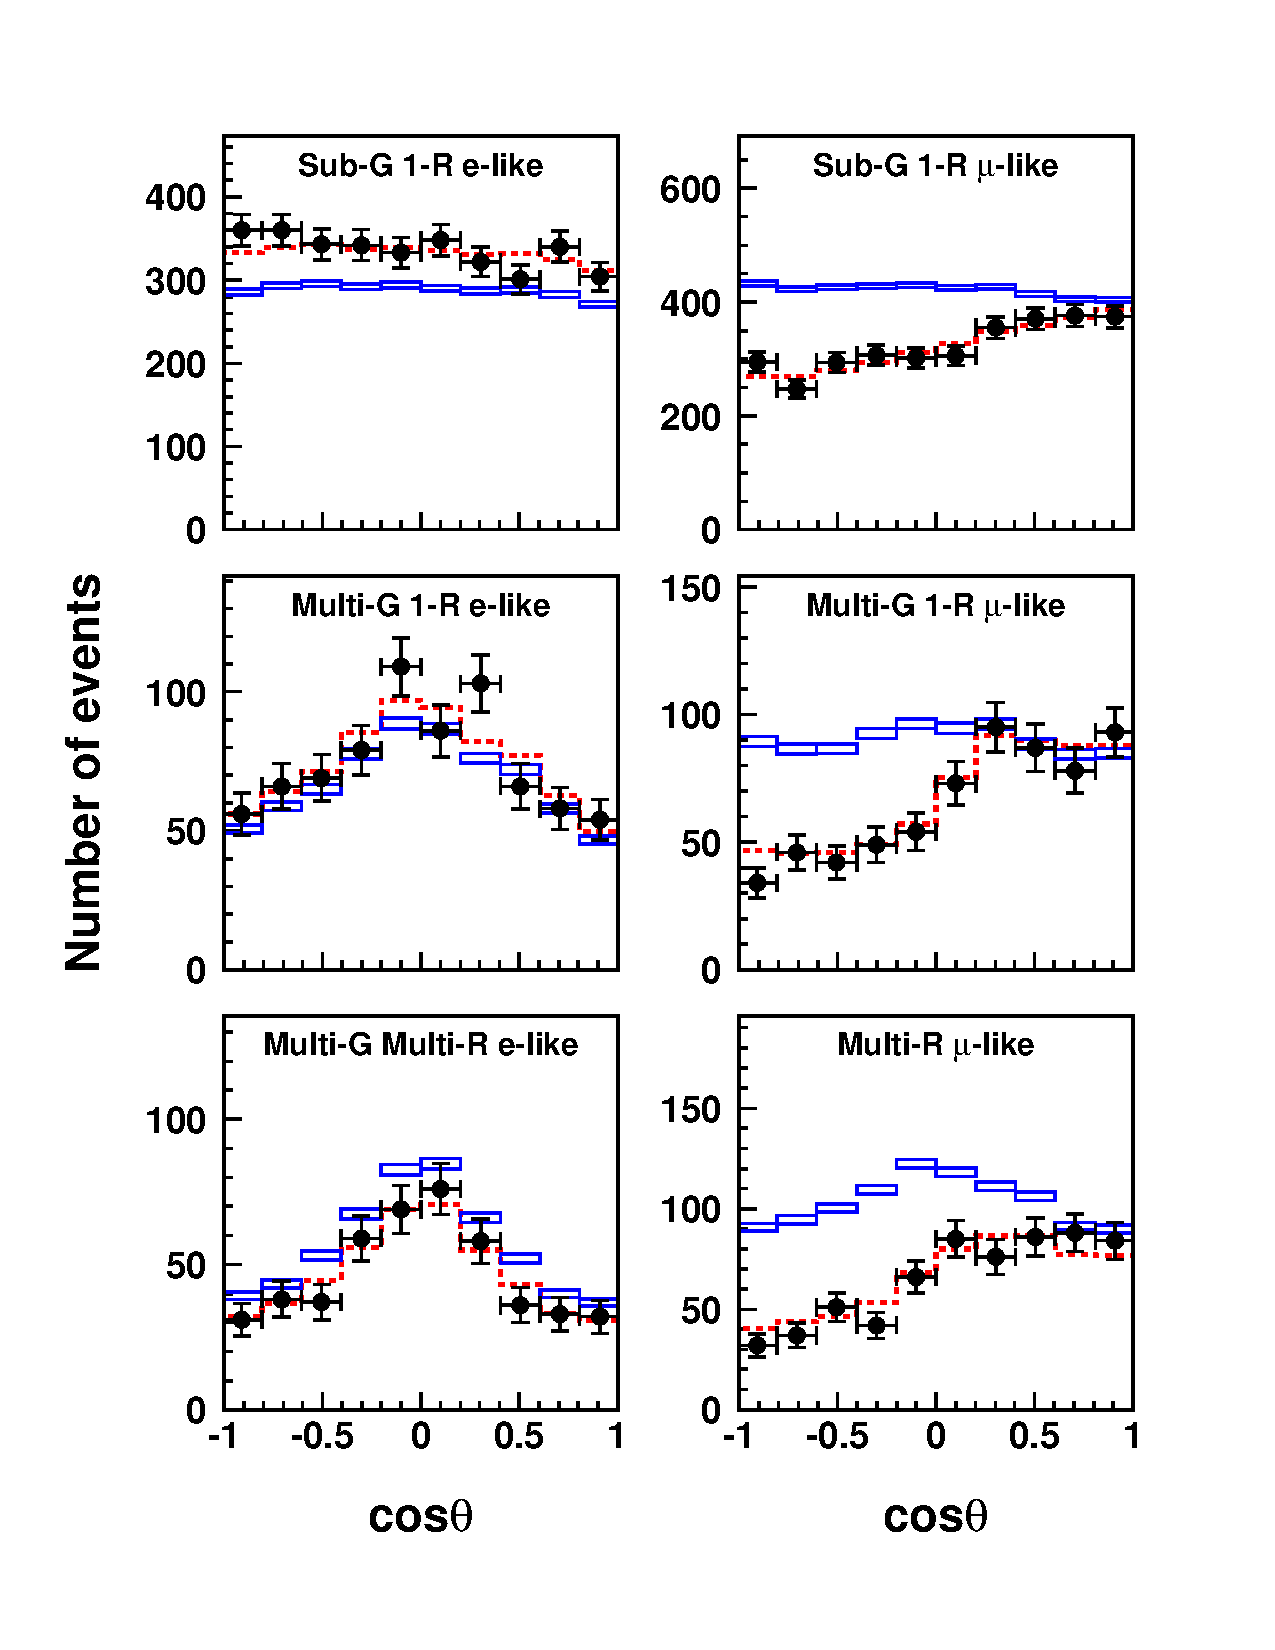
\includegraphics[width=0.6\linewidth]{figures/sk-2006-atm.pdf}
  \caption{Zenith angle distributions of Super-Kamiokande atmospheric neutrino events from \cite{ref:sk-atm-2006}. Fully contained
e-like, $\mu$-like events
are shown for data (filled circles with statistical
error bars), MC distributions without oscillation (boxes)
and
best-fit distributions (dashed). The box height shows the
statistical error.}
 \label{fig:sk-atm}
 \end{figure}

Independently of any accurate predictions of the neutrino flux, the experimental observation of the distributions of Fig.\ref{fig:sk-atm} is sufficient to make a strong case for neutrino disappearance. Indeed, above several GeV, the neutrino flux is isotropic, as the primary cosmic rays are not deflected in a significant way by the geomagnetic field. The observation of a zenith angle dependent deficit of the neutrinos is then a sufficient argument to conclude that these neutrinos undergo a non-standard propagation.  

While in 1998 other hypotheses like decay or decoherence were still open, more recent data from long baseline accelerator experiments have ruled out all explanations apart from oscillations because the alternative hypotheses imply a different L/E behaviour. 
    
The IceCube experiment at the South Pole has recently completed the installation of DeepCore, a denser array of optical modules, aimed at significantly lowering the muon threshold. With data recorded between 2011 and 2014, corresponding to 5074 observed events, they have recently published an analysis of the disappearance of atmospheric $\nu_\mu$  \cite{ref:icecubedis} in the range 10-100 GeV, requiring the zenithal angle to satisfy $\cos theta < 0$,  which has a similar sensitivity to that of Super-Kamiokande (Fig. \ref{fig:icecubeosc}) with the prospects of further improvements. 


\begin{figure}[htbp]
\centering
%\includegraphics[width=0.5\linewidth]{energy_miniboone.eps}
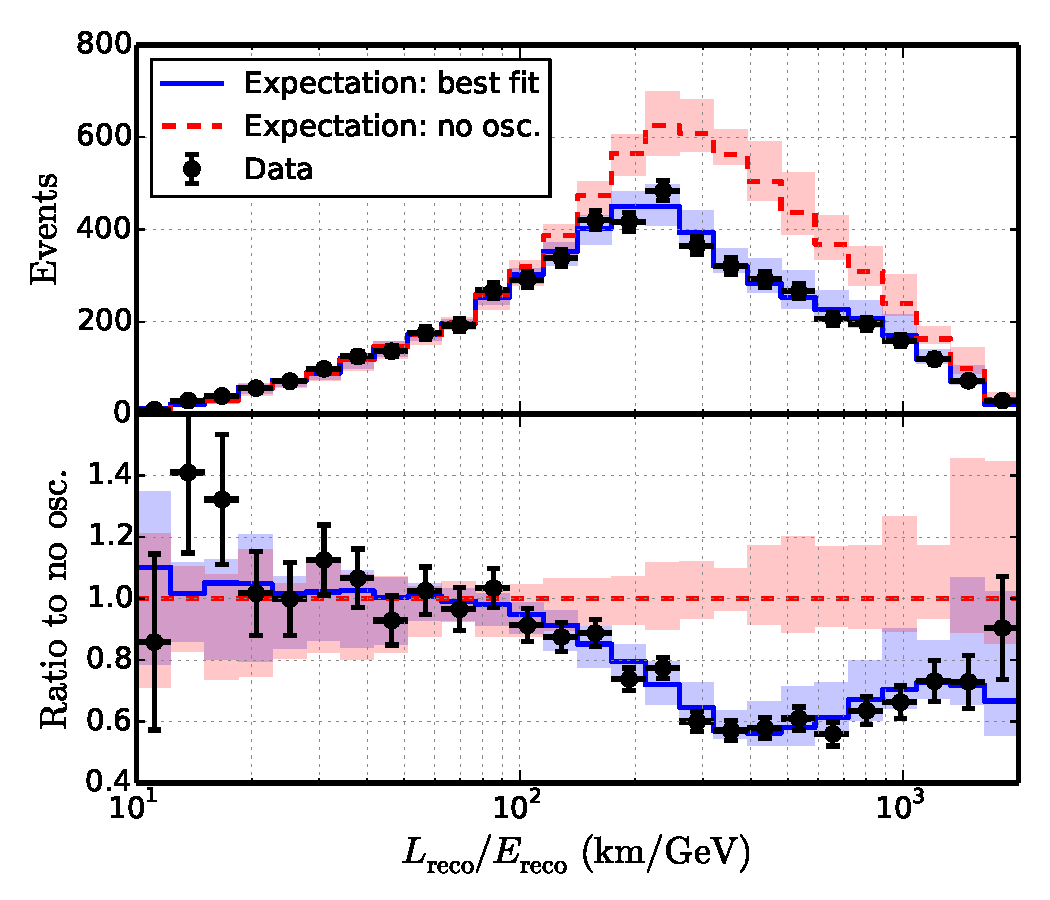
\includegraphics[width=0.6\linewidth]{figures/icecube_osc2014_data_mc_LE.pdf}
  \caption{Distribution of atmospheric neutrino events measured by the IceCube experiment\cite{ref:icecubedis} as a function of
reconstructed L/E. Data are compared to the best fit and
expectation with no oscillations (top), and the ratio of data
and best fit to the expectation without oscillations is also shown
(bottom). Bands indicate estimated systematic uncertainties.}
 \label{fig:icecubeosc}
 \end{figure}


\subsubsection{Long-baseline neutrino beams }

Neutrino beams\cite{ref:kopp} based on particle accelerators have been used since the 1960s, when they provided the evidence for the existence of two types of neutrino, $\nu_e$ and $\nu_\mu$. The general design is based on a high intensity proton beam impinging on a target and producing pions and kaons through interactions on the target nuclei. 
These mesons decay in a dedicated volume downstream of the target, creating mainly a $\nu_\mu$ beam.  

The long baseline beams are based on the so called wide band beam concept. Here the secondary charged mesons are focused using a system of magnetic devices, called horns. The horns, usually with a cylindrical symmetry around the beam, are pulsed with a very intense current in coincidence with the arrival of the beam. 
%The ratio between the primary proton energy and the typical neutrino energy is %at least a factor ten, and the neutrino spectrum extends for about a decade %around this typical energy.  

The flux is tuned in such a way that the phase $\Delta m^2_{32} L/ (4 E)$ reaches $\pi/2$ for the design baseline $L$ and the peak energy $E$, in order to probe the atmospheric oscillation sector with the beam $\nu_\mu$. To do so, the proton energy, the target length and width, the focussing system and the decay volume length and width need to be accurately designed and optimized.   

An off-axis neutrino beam \cite{ref:beavis} relies on the following idea: as the $\nu_\mu$ are mainly produced by the two-body decays of pions, there is a correlation between pion energy $E_\pi$, the neutrino energy $E_\nu$ and the decay angle $\theta$ 
\begin{equation}
E_\nu = \frac{(1-(m_\mu/m_\pi)^2) E_\pi}{(1+\gamma^2 \theta^2) } 
\end{equation}
valid in the limit of small angles.

Neutrinos emitted at a small angle with respect to the pion direction have a distinct narrow spectrum peaking at a much lower energy with respect to the on axis beam. This feature that has been used by the T2K and NOvA experiments, offers several advantages because it avoids the large high energy tail of the on axis beam, thereby reducing some background reactions. 

\begin{figure}[htbp]
\centering
%\includegraphics[width=0.5\linewidth]{energy_miniboone.eps}
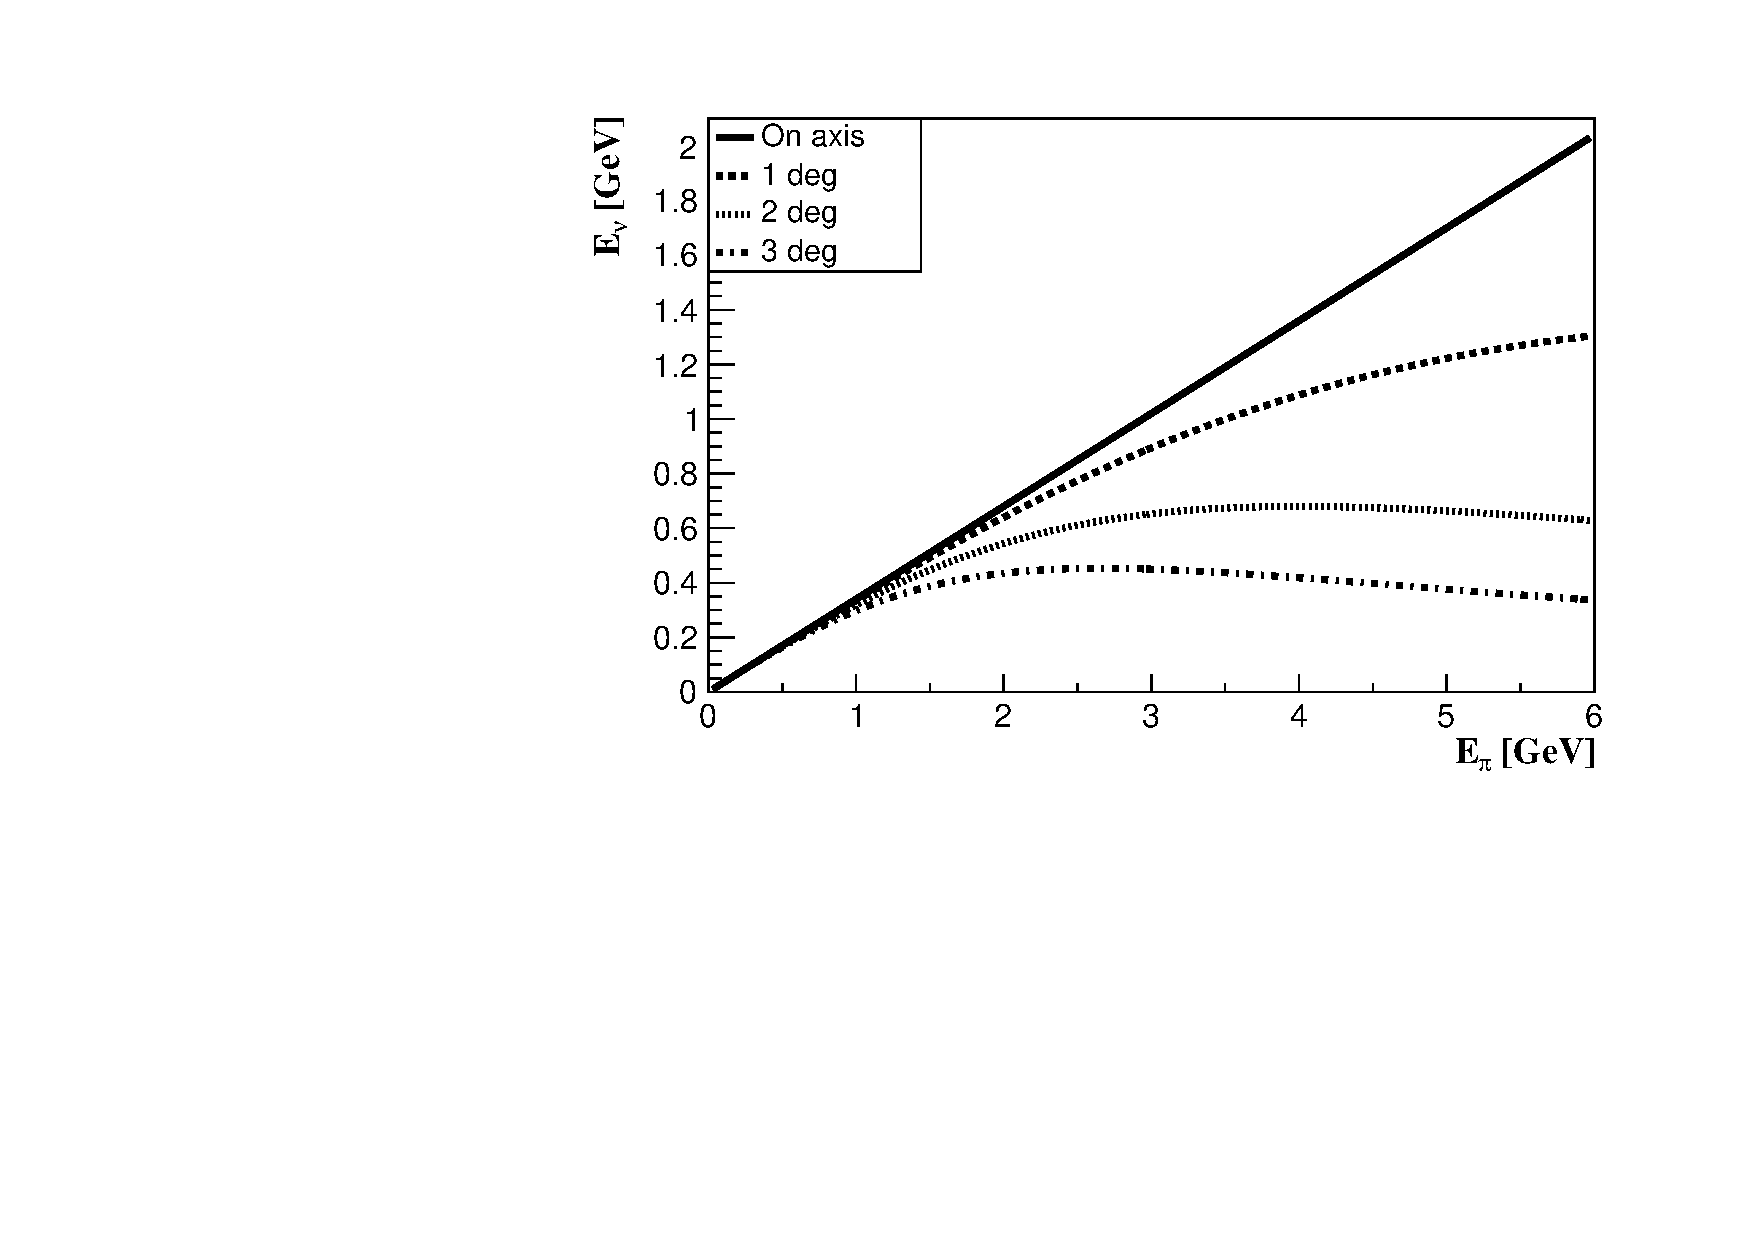
\includegraphics[width=0.6\linewidth]{figures/offaxis.pdf}
  \caption{Neutrino energy as a function of the pion energy for on-axis decays and several off-axis angles. For a non-zero off-axis angle, the neutrino energy reaches a maximum. This feature is currently exploited in the T2K and NOvA experiments.}
 \label{fig:offaxis}
 \end{figure}


As the neutrino beam is a tertiary beam, it is necessary to include in the experimental apparatus monitoring devices to ensure that it is stable in intensity and direction. To this effect, muon detectors, sensitive to the muons produced by the pion decays, are placed close to the end of the decay volume. Moreover, as the neutrino flux and cross-sections and the beam composition are not known with sufficient precision, a near detector is located close to the target station (typically within a few hundred meters). The near detector constrains the neutrino interaction rate, proportional to the product t=of neutrino flux and the cross-section. Moreover, the near detector allows to measure the beam composition and to perform study of several neutrino cross-section.    

Description of T2K beam line if space allows.

\begin{table}
\centering
\begin{tabular}{|c|c|c|c|c|c|}
  \hline
  Exp. & Energy (GeV) & Power (kW) & L (km) & FD mass (kt) & POT \\ 
  \hline
K2K & 30 & & 250 & 22.5 & \\
MINOS & 120 & 700 & 790 & 5.4 &\\
OPERA & 450 & 732 &  & & 1.8 10$^{20}$\\
T2K & 30 & 750 & 295 & 22.5 & 8 10$^{21}$\\
NOvA & 120 & 700& 810 & 14 & \\
HK & 30 & & & & \\
DUNE & 120 & 1200 & 1300 & 40 &\\
  \hline
\end{tabular}
\caption{Parameters of recent and future long baseline experiments. Energy and power refer to the primary proton beam, L is the baseline, FD the mass of the far detector. POT (Proton On Target) represents the integrated dataset as of 2016.}
\end{table}


\subsubsection{Results from long-baseline accelerator experiments K2K MINOS T2K NOVA}

K2K (KEK-to-Kamioka) was the first long baseline neutrino beam, using Super-Kamiokande as its far detector at 290 km from the neutrino production. Operating between 1999 and 2004, it has measured the disappearance of $\nu_\mu$: 112 events were observed, while 158.1$^{+9.2}_{-8.6}$ were expected without oscillation, a 4.3 $\sigma$ effect. This measurement has confirmed neutrino oscillation as the explanation for the atmospheric neutrino disappearance. 

Further precision measurements of the $\nu_\mu \rightarrow \nu_\mu$ were reported by MINOS, T2K and NOvA.

We will here describe in some detail the T2K measurement, the most precise for what concerns the $\theta_{23}$ angle.

\begin{figure}[htbp]
\centering
%\includegraphics[width=0.5\linewidth]{energy_miniboone.eps}
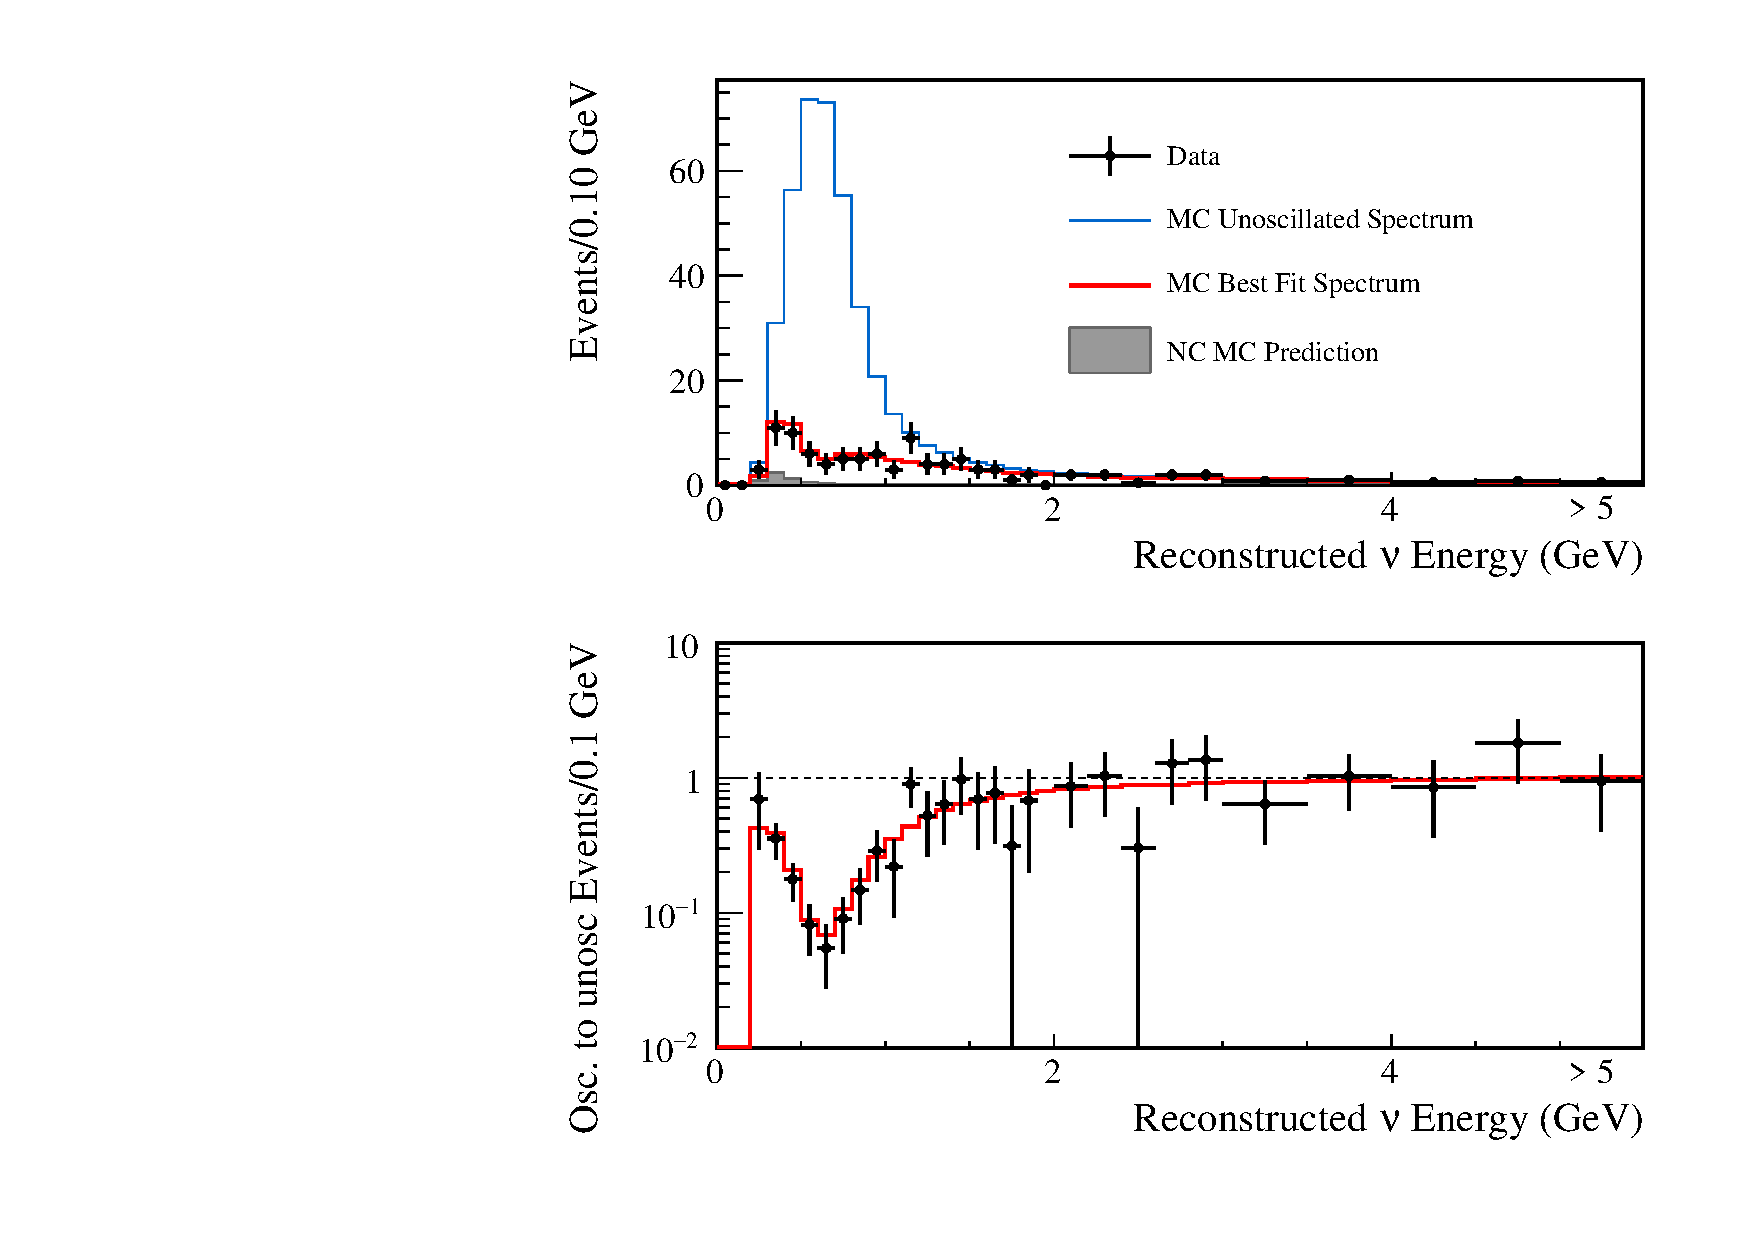
\includegraphics[width=0.6\linewidth]{figures/t2k-disapp.pdf}
  \caption{
Reconstructed $\nu_\mu$ energy spectrum by the T2K collaboration for data, best-fit prediction, and
unoscillated prediction. Bottom: Ratio of oscillated to unoscillated events as a function of
neutrino energy for the data and the best-fit spectrum.
}
 \label{fig:t2kdis}
 \end{figure}

\begin{figure}[htbp]
\centering
%\includegraphics[width=0.5\linewidth]{energy_miniboone.eps}
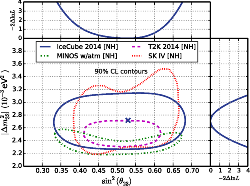
\includegraphics[width=0.6\linewidth]{figures/atm-contour.pdf}
  \caption{
  90\% CL regions in the plane $\Delta m^2 $ versus $\sin^2 (2 \theta_{23}$
  determined by Super-Kamiokande and IceCube-DeepCore using atmospheric neutrinos, and MINOS and T2K using long baseline neutrino beams. 
}
 \label{fig:atm-contour}
 \end{figure}




\subsubsection{Evidence for $\nu_\tau$ appearance}

The OPERA experiment on the CERN to Gran Sasso neutrino beam, taking data between 2008 and 2012, was designed to test the $\nu_\mu \rightarrow \nu_\tau$ appearance hypothesis. The detector is based on the Emulsion Cloud Chamber technique, with 1800 ton of nuclear emulsion detectors in the forms of bricks, each brick being composed of a stack of nuclear emulsion film and lead plates. This target, capable of sub-micrometric track resolution, is devoted to the study of the neutrino interaction vertex and the particles associated to it. The identification of the $\tau$ leptons relies mainly on their characteristic kink (Fig.~\ref{fig:opera}) due to the decay $\tau \rightarrow h \nu_\tau$, or $\tau \rightarrow l \nu_\tau \bar \nu_l$, where $h$ is a charged meson, and $l$ is an electron or a muon. Another signature is related to the decay $\tau \rightarrow 3 h \nu_\tau$ where the short $\tau$ track ends in a three-pronged vertex. The target detectors are complemented by scintillator trackers and muon spectrometers. 

OPERA has observed 5 $\nu_\tau$ candidate events \cite{ref:opera} with a total background of 
$0.25 \pm 0.05$ events, mainly coming from decays of charmed particles. This corresponds to a 5.1 $\sigma$ observation of $\nu_\tau$ production in an oscillated $\nu_\mu$ beam. 

The Super-Kamiokande collaboration has also searched for $\nu_\tau$ appearance in multi-ring events to test the hypothesis of $\nu_\mu \rightarrow \nu_\tau$ oscillations. While the selected sample is affected by large backgrounds, there is an excess of tau-like events in the upward-going direction with a significance of 3.8 $\sigma$, offering a complementary confirmation of the OPERA result.  
 
\begin{figure}[htbp]
\centering
%\includegraphics[width=0.5\linewidth]{energy_miniboone.eps}
%\includegraphics[width=0.6\linewidth]{figures/topology_modified.pdf}
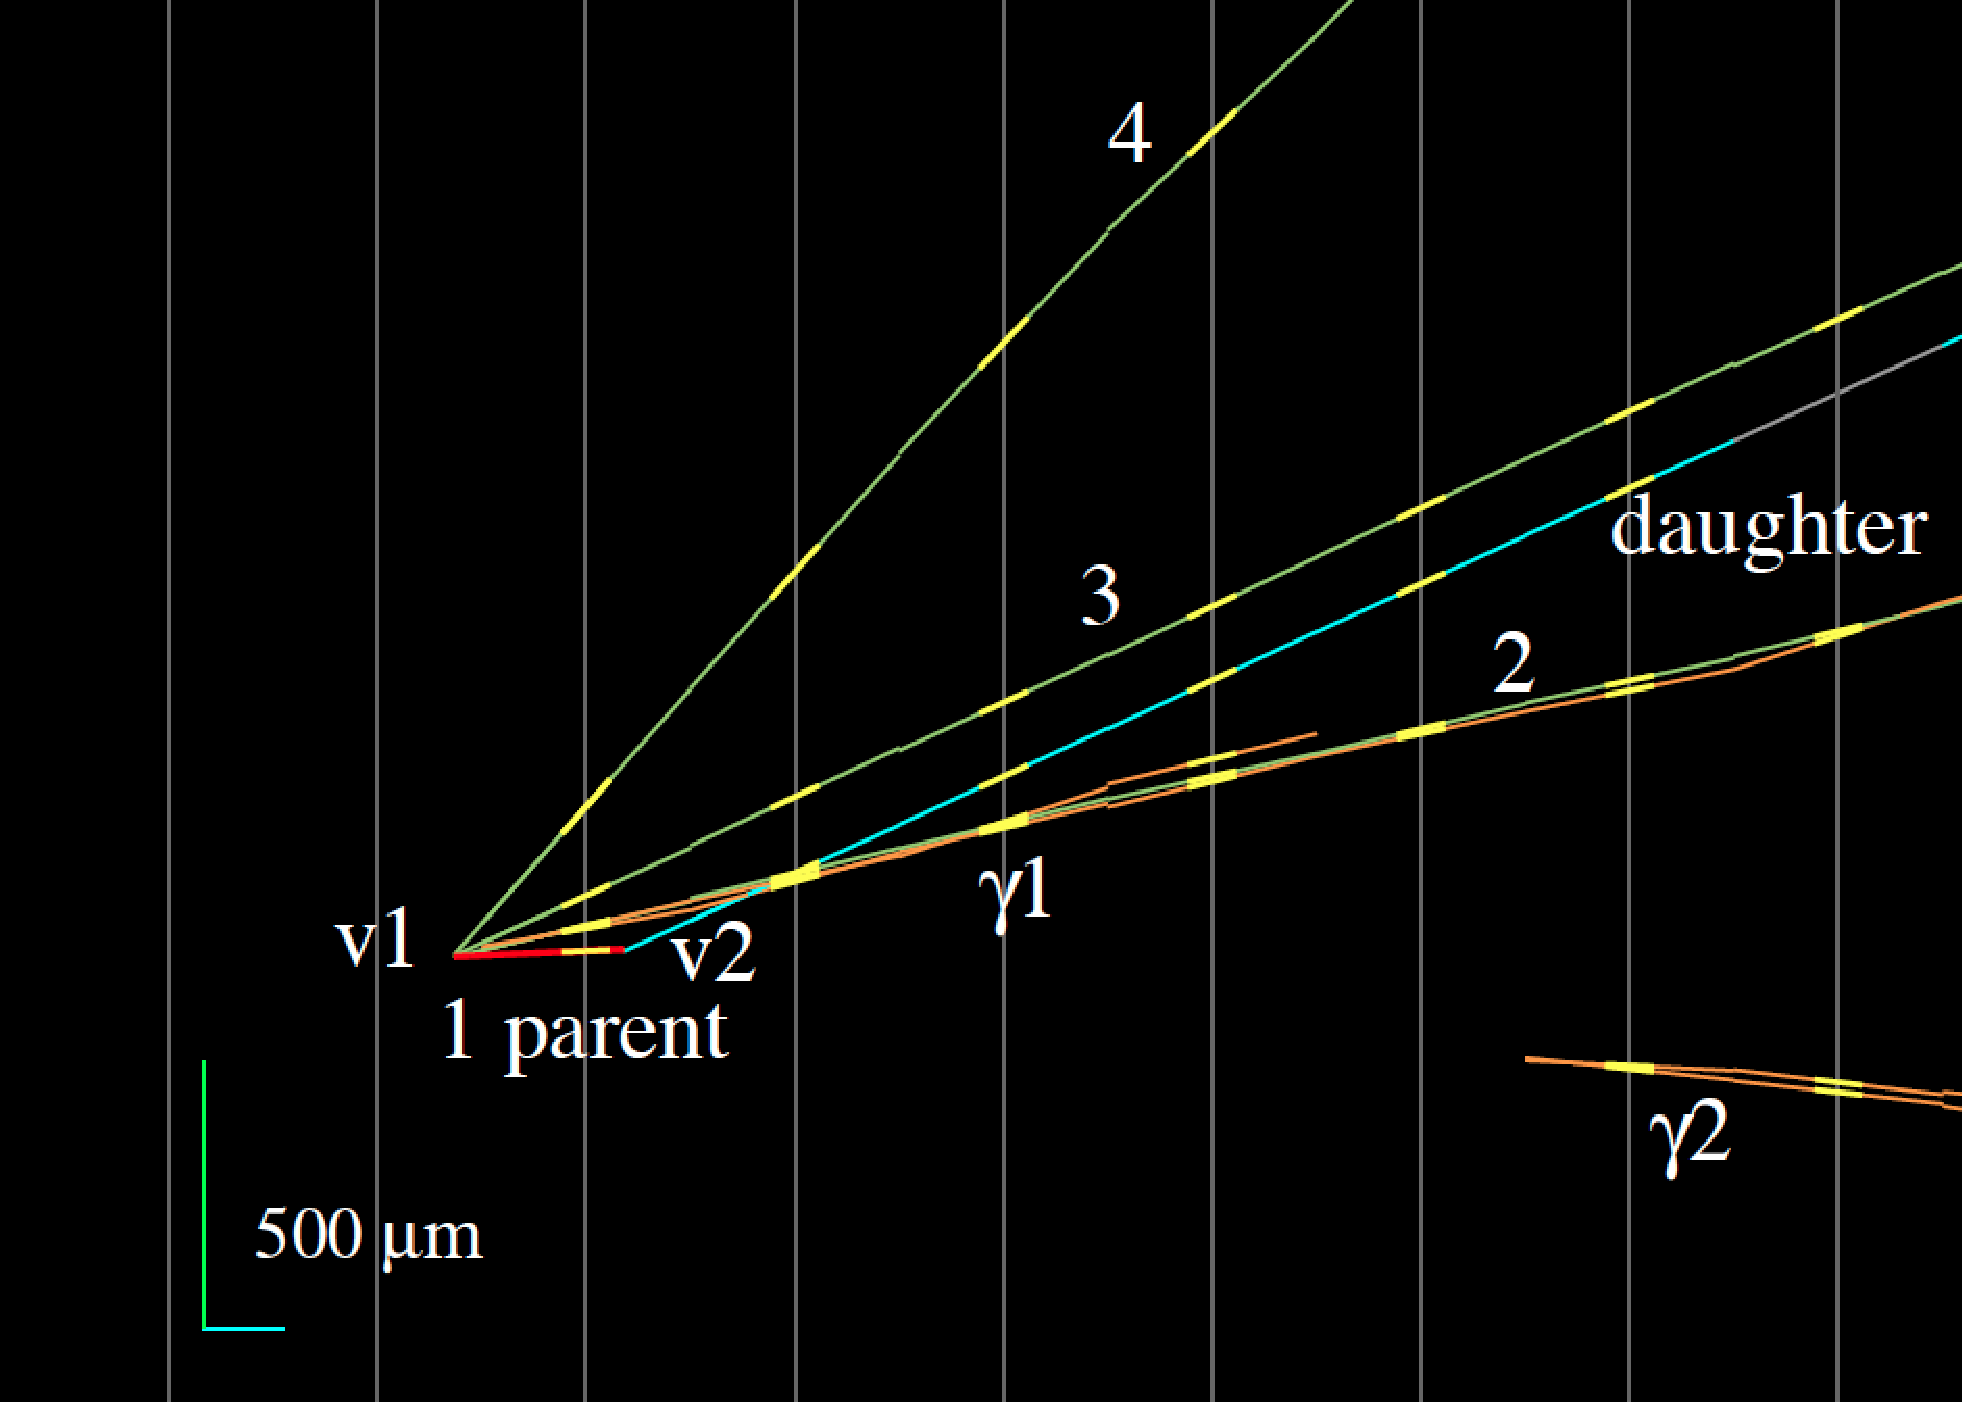
\includegraphics[width=0.6\linewidth]{figures/tau4.pdf}
  \caption{
Event display of the fourth $\nu_\tau$ candidate event from the OPERA 
experiment\cite{ref:opera2} in the
horizontal projection longitudinal to the neutrino direction.
The primary and secondary vertices are indicated as V$_0$ and
V$_1$ , respectively. The kink between the parent and daughter track, a feature of $\tau$ lepton decays, is clearly visible. The yellow stubs represent the track segments as measured in the emulsion films.  
}
 \label{fig:opera}
 \end{figure}

\subsection{The 1-3 sector (MZ)}

\subsection{The 1-3 sector (MZ)}


Solar and atmospheric results are well described by two-flavour mixing models, but we know that there are at least three neutrino flavours and therefore at least three mass eigenstates. The experiments described so-far, while giving robust evidence for neutrino oscillation, do not provide a full picture of 3x3 mixing models. 

In order to fully establish the PMNS matrix it is necessary to measure the last mixing angle, \thint. A non-zero value of \thint is required to have CP violation in the lepton sector. The parameter \thint can be measured by reactor neutrino experiments through the measurement of \nueb disappearance at short baselines ($\sim1~km$) or by long-baseline accelerator experiments by looking for electron neutrino appearance in the \num beam.
Reactor experiments directly measure \thint by observing \nueb disappearance according to the simple equation:

\begin{equation}
P(\nueb \rightarrow \nueb) = 1 - \sin^2 2\thint \sin^2(1.267 \dmsqtwo  L/E)
\end{equation}

This is not the case in long-baseline accelerator experiments for which the \nue appearance probability is a sub-leading effect of the oscillation involving \dmsq in which \num mainly oscillate into \nut. The general expression for \papp is a complicated formula that can be derived considering the formalism for the three neutrino families and depends on a combination of \thint, \dcp and matter effects due to the large amount of matter crossed by neutrinos before reaching the detector. An approximated expression of this probability is:

\begin{eqnarray*}
\papp & = & 4C^2_{13}S^2_{13}S^2_{23}\sin^2\phi_{31} \\
& + & 8 C^2_{13}S_{12}S_{13}S_{23}(C_{12}C_{23} \cos \dcp - S_{12}S_{13}S_{23}) \cos\phi_{32}\sin\phi_{31}\sin\phi_{21} \\
& - & 8C^2_{13}C_{12}C_{23}S_{12}S_{13}S_{23} \sin \dcp \sin \phi_{32} \sin \phi_{31} \sin \phi_{21} \\
& + & 4S^2_{12}C^2_{13} (C^2_{12}C^2_{23} + S^2_{12}S^2_{23}S^2_{13} - 2C_{12}C_{23}S_{12}S_{23}S_{13} \cos \dcp ) sin^2\phi_{21}\\
& - & 8C^2_{13} S^2_{13} S^2_{23} \frac{aL}{4E_{\nu}} (1 - 2S^2_{13} ) \cos\phi_{32} \sin \phi_{31} \\
& + & 8C^2_{13}S^2_{13}S^2_{23}\frac{a}{\dmsqtwo}(1-2S^2_{13})\sin^2\phi_{31} \\
\end{eqnarray*}
\begin{equation}
\label{eq:theta13app}
\end{equation}

where $C_{ij} = \cos \theta_{ij}$, $S_{ij} = \sin \theta_{ij}$ and $\phi_{ji}~= \Delta m^2_{ji} L / 4 E_{\nu}$. The terms that include $a$ are a consequence of the matter effects with $a=2\sqrt 2 G_F n_e E_{\nu}~=~7.56\times10^{-5} [eV^2](\rho/(g/cm^3)(E_{\nu}/GeV)$. The term proportional to cos\dcp is invariant for $\nu$ and \nub whilst the term proportional to sin\dcp change if CP is violated. 
The equivalent term for \pappb can be obtained by reversing the signs of the terms proportional to sin\dcp and to $a$. 

These formulas clearly show the complementarity between reactor and long-baseline experiments. The combination of \nueb disappearance from reactors with the measurement of \nue (and eventually \nueb) appearance in long baseline experiments allows to break the degeneracies and access independentely to \thint, \dcp and the sign of $a$.

In this section we will describe the measurements of \nueb disappearance from Daya Bay, RENO and Double Chooz. In addition the combination with measurement of \nueb disappearance provided by The difference between the two channels clearly show the complementarity between reactor and accelerator experiments that can be combined together to measure \dcp and mass hierarchy.


reactor flux

Bugey et al no disappearance

CHOOZ : theta13 small

DCHOOZ RENO Daya Bay theta13 prec. measurement ND/FD technique

bump and uncertainty flux (anomaly) no impact on theta13

\subsection{ 3 nu effects (MZ)}

\subsubsection{ PMNS model}

data well described by 3nu oscillations (PMNS)

recent global fit (Concha/FL) table

experiment start to be sensitive to 3nu effects

\subsubsection{ long baseline}

T2K and NOVA (effect coupled to MH, NOVA if they publish)

nue appearance senstivity to delta CP (plot)

SK effect in atm due to delta

\subsection{Anomalies (SL)}

LSND numu bar  $\rightarrow$ nue bar  $\rightarrow$ 4th nu

Miniboone inconclusive

reactor anomaly (controversy) - Ga anomaly

tension appearance/disappearance (CDHS Daya Bay Bugey)

3+1 models, bad fits

need for a clarification exp : test of reactor anomaly reactor(SOLID STEREO) + sources (SOX) + accelerators

need to understand the reactor spectrum


\section{Perspectives for future experiments 20pg MZ}
\label{sec:future}


\subsection{Existing projects: T2K NOVA}

T2K statx10 + antinu data no MH

NOVA MH sensitivity (depends on delta)

(where do we add  SK ?)

increased sensitivity to theta23


\subsection{middle term}

JUNO prec measurement of theta12 and Dm21

method NH/IH, critics Parke

depends on E exp resolution, not demonstrated

PINGU/ORCA discussion sensitivity MH (numu->numu vs showers)

INO distinguishes btw numu and numubar status ? 


\subsection{Long term: HyperKamiokande, DUNE}

DUNE new technology LAr 40 kt new beam

decouples CP violation from MH with nu/nubar beam

HyperK 500 kt fiducial (finance ?) upgraded T2K beam

complementarity DUNE/HK

\section{Conclusions}
\label{sec:conc}




%% The Appendices part is started with the command \appendix;
%% appendix sections are then done as normal sections
%% \appendix

%% \section{}
%% \label{}

%% If you have bibdatabase file and want bibtex to generate the
%% bibitems, please use
%%
%%  \bibliographystyle{elsarticle-harv} 
%%  \bibliography{<your bibdatabase>}

%% else use the following coding to input the bibitems directly in the
%% TeX file.

\begin{thebibliography}{00}

%% \bibitem[Author(year)]{label}
%% Text of bibliographic item

\bibitem{ref:Ga2002}
T. Gaisser and M. Honda, Flux of Atmospheric Neutrinos, Ann. Rev. Nucl. Part. Sci. 52 (2002) 153.

\bibitem{ref:midori}
M. Honda, T. Kajita, K. Kasahara, S. Midorikawa  Phys. Rev. D 83 (2011) 123001. 

\bibitem{ref:barr}
G. Barr, et al. Phys. Rev. D 70 (2004) 023006.

\bibitem{ref:fluka}
G. Battistoni et al. Astropart. Phys. 19 (2003) 269.
%\bibitem{ref:}

\bibitem{ref:achar}
C. Achar, et al. Phys. Lett. 18 (1965) 196.

\bibitem{ref:reinesAtm}
F. Reines, et al. Phys. Rev. Lett. 15 (1965) 429.

\bibitem{ref:skatm98}
Y. Fukuda, et al. (Super-Kamiokande Collab.) Phys. Rev. Lett. 81 (1998) 1562.

\bibitem{ref:sk-atm-2006}
J. Hosaka et al., (Super-Kamiokande Collab.) Phys. Rev. D 74, 032002 (2006),


\bibitem{ref:icecubedis}
%M. Aartsen, et al. (IceCube Collab.) Phys. Rev. Lett. 111 (2013) 081801.
M.G. Aartsen et al., Nuclear Physics B 908  161 (2016).

\bibitem{ref:kopp}
S. Kopp, Phys. Rep. 439 (2007) 101

\bibitem{ref:beavis}
D. Beavis et al. 
%“P889: Long Baseline Neutrino Oscillation Experiment at the AGS,”
Report No. BNL-52459, 1995.

\bibitem{ref:k2k}
M. H. Ahn et al, (K2K Collab.), Phys. Rev. D 74 (2006) 072003. 

\bibitem{ref:skatauapp}
Abe K, et al. (Super-Kamiokande Collab.) Phys. Rev. Lett. 110 (2013) 181802.

\bibitem{ref:opera}
N. Agafonova et al. (OPERA Collaboration)
Phys. Rev. Lett. 115 (2015) 121802.

\bibitem{ref:opera2}
A. Di Crescenzo, Nuclear and Particle Physics Proceedings 265–266 (2015) 186–188.

\end{thebibliography}
\end{document}

\endinput
%%
%% End of file `elsarticle-template-harv.tex'.
